\documentclass[11pt,a4paper]{article}

\usepackage[margin=2.4cm]{geometry}
\usepackage{amsmath,amssymb}
\usepackage{booktabs}
\usepackage{array}
\usepackage{tabularx}
\usepackage{graphicx}
\usepackage{siunitx}
\usepackage{xcolor}
\usepackage{microtype}
\usepackage[hidelinks]{hyperref}
\usepackage{caption}
% Keep floats near their first text reference: [section] flushes all pending
% floats at every \section boundary so a figure can never drift into a later
% section, and the relaxed fractions let a figure share a page with text
% instead of being deferred to a float page at the end.
\usepackage[section]{placeins}
\renewcommand{\topfraction}{0.85}
\renewcommand{\bottomfraction}{0.7}
\renewcommand{\textfraction}{0.07}
\renewcommand{\floatpagefraction}{0.8}
\setcounter{topnumber}{3}
\setcounter{bottomnumber}{2}
\setcounter{totalnumber}{5}

\definecolor{accent}{HTML}{2563EB}
\definecolor{accent2}{HTML}{0891B2}
\captionsetup{font=small,labelfont={bf,color=accent}}
\hypersetup{colorlinks=true,linkcolor=accent,citecolor=accent,urlcolor=accent2}
\sisetup{detect-all,per-mode=symbol}
\graphicspath{{figures/}}

\newcolumntype{L}{>{\raggedright\arraybackslash}X}
\newcommand{\tabfont}{\small}

\newcommand{\rT}{\textsf{RSLAB}}
\newcommand{\code}[1]{\texttt{\small #1}}
\newcommand{\nnz}{\mathrm{nnz}}
\newcommand{\bigO}{\mathcal{O}}
\newcommand{\LDLt}{\mathbf{L}\mathbf{D}\mathbf{L}^{\!\top}}
\newcommand{\LU}{\mathbf{L}\mathbf{U}}

\title{\textbf{\textcolor{accent}{RSLAB}}\\[2pt]
\large A Pure-Rust Sparse Direct Solver: Algorithms, Implementation, and Benchmarks}
\author{Milan Rother}
\date{\today}

\begin{document}
\maketitle

\begin{abstract}
\noindent\rT{} is a pure-Rust sparse direct solver with three factorization paths: a
supernodal complex-symmetric $\LDLt$ with Bunch--Kaufman pivoting, an unsymmetric
supernodal/multifrontal $\LU$ with threshold partial pivoting, and a KLU-style path
(block triangular form + per-block Gilbert--Peierls $\LU$) for circuit-shaped systems.
It is generic over the scalar type (\code{f64}, \code{f32}, and their complex
counterparts) and links no external numeric library: the SIMD dense kernels, the
fill-reducing orderings, and the factorizations are all Rust. The analyze phase computes
a-priori peak-memory, work, and runtime predictors as exact functions of the matrix
structure; the default configuration is deterministic and model-free (an exact ordering
race that scores candidates by their true factor fill, the measured kernel knobs, and a
worker count from a one-time cached hardware calibration); and the numeric factorization
is bit-identical regardless of the worker count. A single-precision factor
can precondition a double-precision Krylov solve, recovering the accuracy at half the
factor memory. When the factor is made approximate (static-pivoted or
thresholded) it becomes a preconditioner, and a matching Krylov layer (COCG/COCR,
flexible GMRES, batched multi-RHS block GMRES with within-cycle deflation, and GCRO-DR
subspace recycling) closes the accuracy gap. This report documents the core algorithms,
their implementation, and the measured performance against \textsf{faer}, MKL PARDISO and
Apple Accelerate over a complete-distribution corpus.
\end{abstract}

\section{Scope and architecture}
\rT{} factorizes and solves $Ax=b$ for sparse $A$ that is complex-symmetric (routed to
$\LDLt$), general unsymmetric (routed to $\LU$), or circuit-shaped (routed to the KLU
path). The primary target is the complex-symmetric systems of frequency-domain
electromagnetic and FEM analysis (curl--curl Maxwell problems with lossy media or PML
are complex-symmetric rather than Hermitian), with the KLU path serving the
MNA/SPICE-class operators of circuit extraction. The implementation is stable Rust with
no C/Fortran dependency and no BLAS/LAPACK/METIS linkage, and is exposed to Python
through a thin PyO3 layer that mirrors the Rust surface
(\code{rslab.ldlt}/\code{lu}/\code{klu}/\code{spsolve}).

All paths follow the standard three-phase flow. \emph{Analyze} orders the matrix, builds
the elimination structure, and produces the a-priori predictors; \emph{factor} performs
the numeric decomposition on the ordered, equilibrated matrix; \emph{solve} runs the
triangular substitutions. Analyze is separated from factor at the API level: a symbolic
object (\code{LdltSymbolic}, \code{LuSymbolic}, \code{KluSymbolic}) is produced once and
factors any number of matrices sharing its sparsity pattern, so a frequency sweep or
Newton iteration pays the ordering and symbolic cost once. Across the corpus the numeric
factor dominates the wall-clock, so the tuning and the parallelism target the factor.
The factored solvers implement the crate's \code{Preconditioner} and
\code{Factorization} traits, which is how the direct and iterative layers compose.

\section{Fill-reducing orderings}
\label{sec:ordering}
The ordering determines fill and therefore both factor time and memory. \rT{} implements
three ordering families behind an \code{OrderingMethod} enum and an adaptive dispatcher,
sharing one quotient-graph elimination engine.

\textbf{Approximate minimum degree.} AMD~\cite{amd} selects the pivot of least
approximate external degree from degree-indexed bucket lists over a sliding index
workspace with in-place garbage collection. The update performs aggressive element
absorption, mass elimination, and supervariable detection by adjacency hashing; rows of
degree above $\max(16,\lfloor10\sqrt n\rfloor)$ are deferred to the tail as dense. AMD is the
\code{Auto} pick for very large, very sparse patterns, and a candidate in the race below.

\textbf{Approximate minimum fill.} AMF (HAMF4~\cite{amf,rothberg-minfill}) replaces the
degree score with an approximate fill score
$\mathrm{RMF}(i)=\bigl(\deg(i)(\deg(i)-1+2\deg_{me})-\mathrm{WF}(i)\bigr)/(nv(i)+1)$,
where the working fill $\mathrm{WF}$ is accumulated per eliminated element in 64-bit
integers. It is the \code{Auto} pick for $n\le\num{10000}$ and, in practice, the race's most
frequent winner on grid problems, staying within $1.10\times$ of the reference HAMF4
fill on a \num{183277}-matrix oracle suite.

\textbf{Nested dissection.} A multilevel recursive bisection~\cite{george,metis} driven
by an explicit work stack (no recursion): coarsen, bisect, refine with
Fiduccia--Mattheyses, uncoarsen with projection and refinement. The separator refinement
is a clean-room node-separator scheme (a two-sided node-FM pass over the separator's
boundary with balance-aware gain buckets, projected and re-refined at every level)
rather than a port; on a $40^3$ grid it produces \num{11.24}M factor entries against
\num{12.52}M for MKL METIS. Subgraphs below 200 vertices or splits with a $\ge90\%$ side
fall back to AMD leaves. The bisection seed is itself raced: a small ensemble of seeds is
scored by exact fill and the best kept, deterministically.

\textbf{Dispatch.} \code{OrderingMethod::Auto} routes by cheap structural predicates
(very large and sparse $\to$ AMD; arrow/bordered patterns $\to$ AMF; otherwise a size
rule). The shipped default is \code{AutoRace}, a two-stage \emph{exact} race. Stage one
runs the \{AMD, AMF, RCM\} symbolic prefixes concurrently and keeps the smallest true
factor $\nnz$; stage two admits the nested-dissection candidate only above a work floor
($\num{5e9}$ predicted flops and $n>\num{10000}$), where its analysis cost amortizes
against the factor it saves, and adopts it only on a strictly smaller exact fill. Ties
break deterministically, so the pick is a pure function of the pattern. The race costs
about $4\times$ a single-pass analysis and returns the exact minimum over its candidates
rather than a predicted one.

\section{Symbolic analysis}
\label{sec:symbolic}
From the ordered pattern \rT{} builds the elimination tree and detects fundamental
supernodes, maximal column runs whose row structure differs only by the eliminated
column. Small supernodes are amalgamated to widen the dense fronts that feed the BLAS-3
kernels: nodes with fewer than $\code{nemin}=16$ columns~\cite{ssids} merge with their
parent, using a column renumbering that re-postorders the tree so a desired parent--child
merge becomes structurally adjacent. Column counts from a depth-first tree walk drive the
factor-size estimate.

\emph{Relaxed} amalgamation~\cite{ashcraft} merges an adjacent child within a width
and extra-row budget, padding the merged front with explicit zeros to trade fill for
higher-rank Schur updates. It is available (\code{with\_relax}) and off by default. The
padded rows are structurally zero, but the numeric path carries them through every update
as arithmetic and as memory traffic, so the trade is favourable only when the padding is
small relative to a front that is already wide. On grid operators, whose fundamental
supernodes are narrow and numerous, it is not: a $145^2$ convection--diffusion grid has
\num{3878} fundamental supernodes against 277 relaxed ones at identical output fill, and
factors $3.4\times$ slower with the relaxation on. Over the 18-matrix corpus the default
is \num{0.654} in geomean factor time against relaxed merging, at identical or lower
fill.

\section{Numeric factorization}
\label{sec:numeric}

\subsection{Equilibration}
Before factoring, $A$ is symmetrically equilibrated as $\hat A=DAD$ with
$s_i=1/\sqrt{\max_j|A_{ij}|}$ in one pass over the lower triangle; the real, symmetric,
positive diagonal preserves complex symmetry and the pivot signs and tolerates zero
diagonals (saddle-point systems). The $\LU$ path applies a two-sided $\hat A=D_rAD_c$;
iterative Ruiz and MC64 matching-based scaling are selectable alternatives.

\subsection{Supernodal left-looking \texorpdfstring{$\LDLt$}{LDLt}}
The default symmetric path assembles one dense panel per supernode, updates it by every
previously factored descendant (\code{cmod}: pull the descendant's columns, apply its
block-diagonal $D$, subtract the rank update, a scalar triple loop below a flop
threshold, a SIMD GEMM above), then factors the fully-summed block in place (\code{cdiv})
by a blocked Bunch--Kaufman partial factorization~\cite{bunchkaufman} with panel width
64. For complex-symmetric $A$ the kernel is the real \code{sytf2} control flow with
magnitudes $|z|$ and no conjugation; the pivot threshold is
$\alpha=(1+\sqrt{17})/8$, pivot selection is bounded to the supernode's fully-summed
rows, and a $2\times2$ block is rejected as singular when
$|d_{11}d_{22}-d_{21}^2|<\varepsilon\max(|d_{11}|,|d_{21}|,|d_{22}|)^2$ with
$\varepsilon=10^{-14}$, bounding the element growth injected into the trailing update.

Transient memory is controlled by \emph{panel freeing}: every supernode carries a
reference count of the ancestors that will still update from it, and when a \code{cmod}
decrements it to zero the panel is compacted into its final CSC fragment and the dense
buffer released (acquire/release atomics make this safe under tree parallelism). The
resident data is the compact factor plus only the live panels. Sibling subtrees factor
concurrently in a scoped rayon pool of caller-set width; per-node GEMMs parallelize above
their flop thresholds.

\subsection{Multifrontal path}
The alternative multifrontal schedule~\cite{duffreid,liumf} assembles a dense frontal
matrix per supernode from its eliminated columns and its children's contribution blocks
(CBs), factors the fully-summed part, and passes the Schur complement up as its CB. A
work-stealing tree recursion factors children in parallel; each CB is freed the moment it
is extend-added into the parent, and where the CB stack is large children are reordered
by Liu's $(\text{peak}-cb)$ rule~\cite{liu86}, a scheduling hint that changes neither
numbering nor fill. The front is denser and more BLAS-3-rich than a left-looking panel
but carries a higher transient peak, which is why both schedules ship and the choice is
per matrix.

\subsection{Unsymmetric \texorpdfstring{$\LU$}{LU}}
General matrices reuse the symmetric analysis machinery on the symmetrized pattern
$A\cup A^{\!\top}$ and ship both numeric schedules. The default supernodal left-looking
$\LU$ uses UMFPACK-style~\cite{umfpack} threshold partial pivoting: the diagonal
candidate is kept when $|a_{jj}|\ge u\,|a_{\mathrm{colmax}}|$ with tunable
$u=\code{pivot\_u}$ (default $0.1$); $u=1$ recovers full partial pivoting, $u=0$ keeps
the natural order and skips the pivot search (the static fast path for fixed-pattern
sequences). The multifrontal $\LU$ factors each front by a blocked right-looking
\code{getrf} with unrestricted partial pivoting over the fully-summed rows. $L$ is stored
CSC (unit lower), $U$ CSR; the column permutation is the fill-reducing ordering and a
separate row permutation records the interchanges.

\subsection{KLU path for circuit-shaped matrices}
\label{sec:klu}
Circuit-class operators (MNA/SPICE: extremely sparse, unsymmetric,
near-triangularizable) defeat supernodal methods: their irreducible blocks are far too
small for BLAS-3 fronts to pay off. \rT{} therefore ships a third path following
SuiteSparse KLU~\cite{klu}, reimplemented in pure Rust.

\emph{Analyze} permutes to block \emph{upper} triangular form (BTF). A maximum
transversal pairs every column with a row holding a structural nonzero (an incomplete
matching proves the matrix \emph{structurally} singular before any numeric work), and
Tarjan's SCC algorithm on the matched digraph, emitted in reverse topological order,
yields the symmetric permutation under which every entry outside the irreducible diagonal
blocks lies above them. Two transversal algorithms ship, the MC21-style augmenting-path matching with
per-column lookahead and Hopcroft--Karp~\cite{hopcroftkarp}; a maximum matching is not
unique, and the choice changes the block structure. Both candidates are therefore scored
by the pattern-only Gilbert--Peierls fill count of the blocks they induce, and the
smaller wins. A diagonal-repair pass then routes the matching through off-diagonal pivots
where that keeps the diagonal structurally nonzero, which removes a fill cascade seen
under row scaling. AMD orders each block on its symmetrized pattern. Fill is confined to
the diagonal blocks; the off-block entries are never factored and enter only the block
back-substitution.

\emph{Factor} runs a left-looking Gilbert--Peierls $\LU$ per block: for each column a
depth-first reach over the pattern of the $L$ columns factored so far yields the fill
pattern in topological order, so the numeric work is proportional to the flop count.
Threshold partial pivoting prefers the (structurally nonzero) diagonal unless it falls
below $10^{-3}$ of the column maximum; row-max scaling equilibrates the rows first.
Results are \textbf{bit-identical across runs and thread counts} in every mode, which is
what lets the path double as the determinism arbiter for the supernodal ones.

Two levels of parallelism sit behind that guarantee, both gated by one principle: a
\emph{work floor} (the overhead is real and is never bypassed) and a \emph{concurrency
ratio} of at least two (an exact Amdahl bound across blocks, the mean elimination-DAG
level width within a block, which also bounds the worker count). Above the gate, the
independent BTF diagonal blocks factor concurrently with a two-phase spliced output.
Refactorization additionally pipelines the columns \emph{inside} a dominant irreducible
block in the manner of NICSLU~\cite{nicslu}: worker-owned column ranges on the frozen
elimination DAG, with just-in-time spin-waits on per-column ready flags instead of level
barriers, on OS threads rather than a work-stealing pool (a spinning task must not starve
the column owner it waits for). That is worth \numrange{2.0}{2.9}$\times$ on the
work-heavy SuiteSparse circuit matrices (rajat15, twotone, ASIC\_100ks, onetone1) and
changes no bit of the result.

\emph{Refactor} is the path's distinctive fast lane: for a new value set on the
\emph{same} pattern (frequency sweep, time stepping, Newton), the stored pattern and
pivot sequence are replayed with no symbolic work and no pivot search; a changed pattern
is detected and rejected exactly, and a frozen pivot that becomes zero fails cleanly so
the caller can re-factor with pivoting. The symbolic object also carries an exact
a-priori fill/flop estimator (a pattern-only Gilbert--Peierls pass under the
diagonal-pivot assumption, computed lazily and cached), mirroring the estimators of the
other two paths.

\subsection{Static pivoting and preconditioner mode}
The \code{ZeroPivotAction} policy governs near-singular pivots on the $\LDLt$/$\LU$
paths: \code{Fail} (default) returns a rank-deficiency error, \code{PerturbToEps} lifts
any sub-floor pivot to the floor while preserving its phase, so the factorization
satisfies $\LDLt=A+\Delta$ with bounded $\Delta$ and never fails. Together with
threshold dropping (\code{drop\_tol}: incomplete factors) and \code{f32} mixed
precision, this never-fail factor is the preconditioner the Krylov layer consumes.
The KLU path never perturbs: a vanishing pivot is a hard, attributed error.

\subsection{Iterative refinement and what it certifies}
\label{sec:refine}
A solve can be refined against the original matrix, and what counts as converged
is the caller's to state: a policy object names the step budget, the target
and the measure, and every entry point returns the achieved backward error
rather than only the step count. With $r=b-Ax$ the two measures are the normwise
$\omega=\|r\|_\infty/(\|A\|_\infty\|x\|_\infty+\|b\|_\infty)$ and the
componentwise $\omega=\max_i|r_i|/(|A||x|+|b|)_i$, the backward errors of
$(A+\delta A)x=b+\delta b$ under $\|\delta A\|\le\omega\|A\|$ and
$|\delta A|\le\omega|A|$ respectively. The componentwise one is the default and
the stricter: a row scaled far below the matrix norm can carry a large relative
error in its own equation while contributing nothing to the normwise ratio, so a
normwise stop certifies solutions a componentwise stop rejects. Refinement is not
monotone on ill-conditioned systems, so the iterate returned is the best measured
one, and a non-finite iterate never certifies. The same contract and the same two
formulas serve the $\LDLt$, $\LU$ and KLU paths; in-place entry points refine a
caller-owned buffer without allocating. The Krylov layer keeps its own stop test
on the true relative residual, a weaker quantity than either backward error.

\section{A-priori predictors}
\label{sec:pred}
The analyze phase computes a set of predictors as \emph{exact functions of the symbolic
structure} and the scalar size $v$, before any numeric work, the basis of the memory
guarantee, the heuristic configuration pick, the thread policy, and the resource planner of
Sec.~\ref{sec:sil}.

\textbf{Per-path peak memory.} The factor size is $\text{factor\_nnz}\cdot(v+8)$, a
structural upper bound (cancellation can only lower it). The transient peak is bounded
separately per schedule. For the left-looking path, a reference-count simulation of the
panel-freeing schedule walks the postorder, adds each panel as it is assembled, frees it
when its refcount reaches zero, and records the running maximum of live panels plus
already-compacted factor, the floor the solver actually operates at; a conservative
whole-run bound adds all panels, the input, and a scratch term
$\tfrac14(\text{panels}+\text{factor})+\SI{32}{\mega\byte}$ for the per-thread
\code{cmod}/\code{cdiv} buffers. For the multifrontal path a level-parallel model takes,
per assembly-tree level, the front sizes $\sum\text{nrow}^2v$ plus that level's child
contribution blocks, times $\tfrac75$ for work-stealing overlap. Over the corpus both
bounds hold at an estimate/measured ratio of $\approx1.3$ in geomean
(Fig.~\ref{fig:membreak}); the panel-freeing floor is the tighter quantity the
resource planner of Sec.~\ref{sec:sil} budgets against. The KLU path carries the same contract: a pattern-only
Gilbert--Peierls pass (Sec.~\ref{sec:klu}) gives its fill and flops exactly under
diagonal pivoting.

\begin{figure}[htbp]
\centering
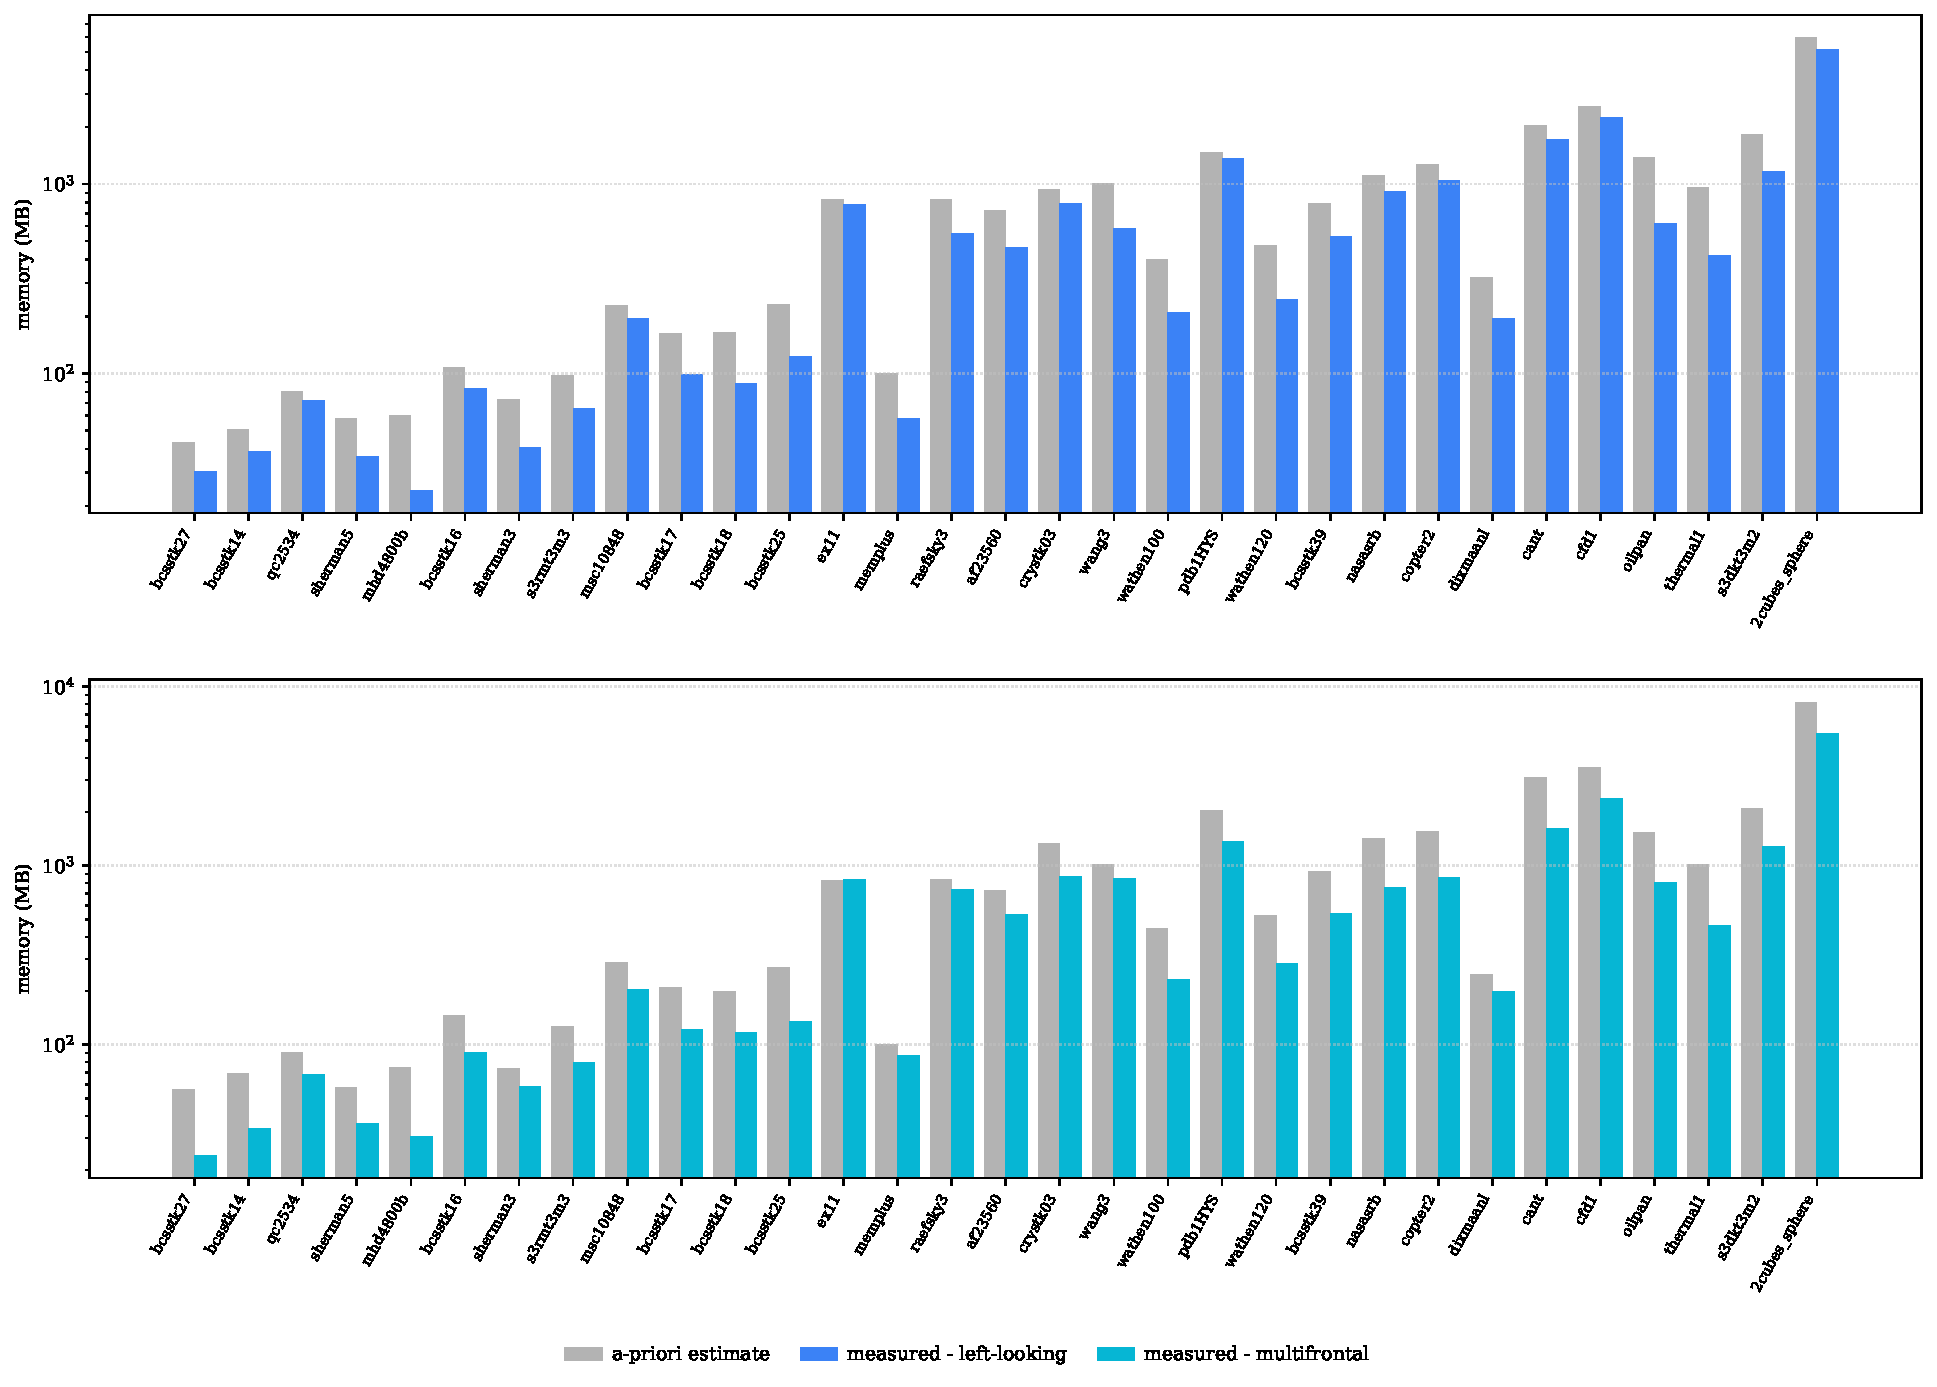
\includegraphics[width=\textwidth]{memory_breakdown.pdf}
\caption{A-priori memory estimate (conservative bound and panel-freeing floor) vs.\ the
measured peak, per RSLAB path. The estimate does not under-predict.}
\label{fig:membreak}
\end{figure}

\textbf{Work, runtime, and threads.} The geometric work
$\text{factor\_flops}=\sum_s\text{nrow}_s^2\,\text{ncol}_s$ is a type-independent proxy;
the thread-aware runtime estimate is
\begin{equation*}
\max\!\Big(\frac{\text{critical\_path\_flops}}{r},\
\frac{\text{factor\_flops}}{r\cdot\text{speedup}}\Big),\qquad r=\text{gflops}\cdot10^9,
\end{equation*}
where the first term is an Amdahl floor from the assembly tree's longest leaf-to-root
chain, so a critical-path-bound matrix does not benefit from more workers. The
single-thread rate and parallel speedup come from a one-time hardware calibration cached
by machine fingerprint; a learned additive residual on the speedup curve (ridge
regression on dimensionless structure features, dominated by
$\text{critical\_path}/\text{factor\_flops}$) cuts the held-out speedup error by
$\sim26\%$. A thread-count predictor caps thin/narrow problems at two workers and small
ones at four, landing within $\sim10\%$ of the per-matrix optimum in geomean (a fixed
two-worker budget is off by $\sim50\%$).

\section{Determinism and the shipped default}
\label{sec:tuner}
Three determinism properties hold. The numeric factor is bit-identical regardless of
worker count: parallel subtrees and GEMMs write disjoint blocks and every reduction sums
in a fixed order, so the thread count is a performance parameter only (the parallel
multi-RHS solve is likewise bit-identical to serial). The analyze-phase choices are
deterministic functions of the pattern. And the resource planner is a pure function of
its inputs. The pivot sequence is value-dependent; $\code{pivot\_u}=0$ (or the KLU
refactor) freezes it across same-pattern refactorizations.

The shipped default configuration is deterministic and model-free: the exact
two-stage ordering race of Sec.~\ref{sec:ordering}, the measured default kernel knobs,
and, after a one-time cached hardware calibration, a critical-path-aware worker count
from the calibrated cost model. Every input to the pick is an exact a-priori quantity;
nothing is modeled, and nothing is measured implicitly at solve time.

Mixed precision enters through the preconditioner rather than through a separate
solver: an \code{f32} factor at half the memory
(\code{LowPrecisionPreconditioner}/\code{LowPrecisionLu}) preconditions an
\code{f64} Krylov solve, GMRES-IR in the sense of Carson--Higham~\cite{carsonhigham}
with the working precision fixed at \code{f64}. On the reference class the
single-precision factor runs $1.64\times$ the double one.

\section{Solver-in-the-loop and resource governance}
\label{sec:sil}
\rT{} is built to run \emph{inside} an outer loop (a frequency sweep, adaptive mesh
refinement, a Newton or time-stepping iteration, many concurrent extractions) rather
than as a one-shot black box, and three mechanisms carry that model. First, analyze and
factor are separate phases: a symbolic object factors any number of matrices sharing its
pattern, so a same-pattern sequence pays the ordering and symbolic cost once (and on the
KLU path the numeric refactor also skips the pivot search). Second, every factorization
runs in a \emph{scoped} thread pool of caller-set width, so many concurrent solves
coexist without oversubscribing the machine, and a factored preconditioner hands its
thread policy to the Krylov layer so factor and solve share one concurrency budget.
Third, the resource planner \code{tuning::plan} turns a memory estimate, a budget (a
memory ceiling and a thread budget), and the cached calibration into a plan (a
predicted peak, a predicted runtime, and a fits/does-not-fit decision) as a pure
function of its inputs. Because the memory estimate of Sec.~\ref{sec:pred} is an upper
bound rather than a sample, a scheduler can pack concurrent solves against a memory
ceiling without extra safety margin, fail fast before allocating, or switch to an
approximate factor when the exact one cannot fit; and because per-solve peaks and
runtimes are predicted, the aggregate footprint and makespan of a batch are computable
before the batch runs. Per-call diagnostics (stage timings, fill, the attached estimate)
close the loop after the fact, estimate against measured.

A fourth mechanism bounds the loop in time: the numeric factorization is
cancellable. The caller owns an \code{AtomicBool}, arms it on the settings, and
\rT{} polls it at supernode, dense-panel and BTF-block boundaries, returning
\code{Interrupted} on the first observation. The library only ever reads the
flag, so re-arming belongs to the caller, and taking a flag rather than a
deadline keeps the solver clock-agnostic: wall-versus-CPU-versus-budget policy
stays with the host that owns the deadline. Without it a host cannot enforce a
time budget it can be smaller than a single factorization, because control never
returns while one runs. The factors after an interrupt are invalid exactly as
after any failed factor, no partial result is promised, and the symbolic
analysis is not interruptible. Unarmed, the poll is one \code{Option} branch
that touches no atomic and measures within noise ($1.007$, $1.012$, $0.998$ on
the reference matrices).

\section{Preconditioned and recycled Krylov layer}
\label{sec:iterative}
When the factor is approximate, accuracy is recovered by iteration. The iteration and
the preconditioner are decoupled by two traits: \code{LinearOperator} supplies
$y\leftarrow Ax$ and a block $Y\leftarrow AX$ (an explicit matrix, or matrix-free;
an FMM/MoM operator with \rT{} factoring only the sparse near-field), and
\code{Preconditioner} supplies $z\leftarrow M^{-1}r$ and a block apply that a factored
solver implements through the parallel \code{solve\_many} (a
\numrange{8}{19}$\times$ wide-RHS speedup the block Krylov methods inherit).

\textbf{Complex-symmetric short recurrences.} For $A=A^{\!\top}$ the methods of choice
are COCG~\cite{cocg} and COCR~\cite{cocr}: structurally CG/CR but with every inner
product in the unconjugated bilinear form $x^{\!\top}y$. A zero bilinear denominator is
reported as a deterministic breakdown with the best iterate, never a division by zero.

\textbf{Flexible GMRES.} For general operators, restarted GMRES~\cite{saadschultz} in
the flexible variant~\cite{fgmres}: the preconditioned Arnoldi vectors $z_j=M^{-1}v_j$
are kept as a second basis and $x\mathrel{+}=Zy$, which saves one $M^{-1}$ solve per
restart cycle and admits a varying preconditioner. Orthogonalization is MGS with a
conditional DGKS~\cite{dgks} second pass. Each cycle measures the \emph{true} residual
$\|b-Ax\|$, the only reliable stop test on ill-conditioned near-field operators,
and a Hessenberg-diagonal guard truncates the least-squares solve to its
well-conditioned prefix, so a rank-deficient cycle reports non-convergence instead of
injecting NaN.

\textbf{Block GMRES.} The multi-RHS solver drives $s$ right-hand sides in lockstep so
matvec and preconditioner are issued once per step as block applies. Each right-hand
side keeps its own Arnoldi basis (batched-independent; a shared-subspace block Krylov
method is future work), which lets a column \emph{deflate} out the moment it converges
including mid-cycle, compacting the batched applies to the still-active width. The
panel orthogonalization is block CGS2~\cite{giraud,barlow}: two panel-wide sweeps,
BLAS-3 intensity, parallelized in fixed row chunks and therefore bit-identical across
thread counts. Measured on preconditioned convection--diffusion ($n=\num{40000}$,
complex), BCGS2 scales to $\sim2.2\times$ at 12 cores where the per-RHS MGS path is
flat-to-negative, and per-RHS cost stays near-flat in the block width.

\textbf{GCRO-DR subspace recycling.} For sequences of related solves,
GCRO-DR~\cite{gcrodr,morgan} retains the $k$ harmonic-Ritz vectors of smallest value,
the near-invariant subspace that governs restarted-GMRES stagnation, and deflates them
across restarts within a solve, and recycles them across solves through an opaque
handle refreshed in place. The subspace only \emph{shapes} the Krylov space: the outer
true-residual test stays authoritative, every recycle step degrades gracefully to plain
FGMRES, and $C=\tilde AU$ is recomputed each solve so the split stays exact when $A$ or
$M$ drift. On a stagnation-spectrum sequence of 8 solves ($n=\num{20000}$), recycling
cuts the cumulative iteration count $6.4\times$ versus cold starts ($2.9\times$ on the
first solve alone) for a $1.5\times$ wall-clock reduction. Warm starts ($x_0$), an
adaptive restart length that keeps the up-front Arnoldi basis under a memory budget, and
\code{f32} mixed-precision preconditioning (\code{LowPrecisionPreconditioner} /
\code{LowPrecisionLu}) complete the layer.

\section{Benchmarks}
\label{sec:eval}
All cross-solver figures come from the \code{bench\_suite} engine over a
complete-distribution corpus: structured-grid generators (curl--curl Maxwell,
shifted Helmholtz, Stokes/KKT saddle-point, convection--diffusion over the grid-P\'eclet
range, BEM/MoM near-field kernels) plus the complex SuiteSparse~\cite{suitesparse}
matrices, 8k--125k DOFs, \code{Complex<f64>}, measured in one run on a quiet 12-core
machine, so the cross-solver ratios carry no run-to-run drift. RSLAB runs its shipped
default (the exact ordering race and the calibrated worker count); each path is compared
on its own class against its own PARDISO mtype~\cite{pardiso} and faer~\cite{faer}.
This corpus was measured with RSLAB v0.27 on a 12-core x86 machine; the Apple
measurement of Sec.~\ref{sec:apple} carries the current version.

\subsection{Scaling and accuracy}
Figures~\ref{fig:h2h_ldlt} and~\ref{fig:h2h_lu} plot factor time and peak memory against
$\nnz$ with per-solver power-law fits; Table~\ref{tab:scaling} gives the head-to-head
geomean ratios. \rT{} sits between the two on both paths: faster than the
pure-Rust faer, moderately behind the hand-optimized MKL PARDISO
($5.6\times$ sym / $5.1\times$ unsym). The heuristic pick's win over the fixed
default is visible as a gap that widens with problem size (largest on the big
matrices where a mispicked ordering costs most) and on the symmetric path
never comes at a memory cost. On accuracy
(Fig.~\ref{fig:residual}), 24 of 31 corpus matrices factor to a relative residual below
$10^{-8}$, matching PARDISO and ahead of faer; the exact $\LDLt$ declines a handful of
indefinite saddle-point matrices rather than returning a degraded solution. The
determinism and equivalence properties were validated over 180 SuiteSparse matrices:
right-looking vs.\ multifrontal, both emit modes, parallel vs.\ serial front
subtraction, and the 32-bit compressed factor are all bit-identical.

\begin{figure}[htbp]
\centering
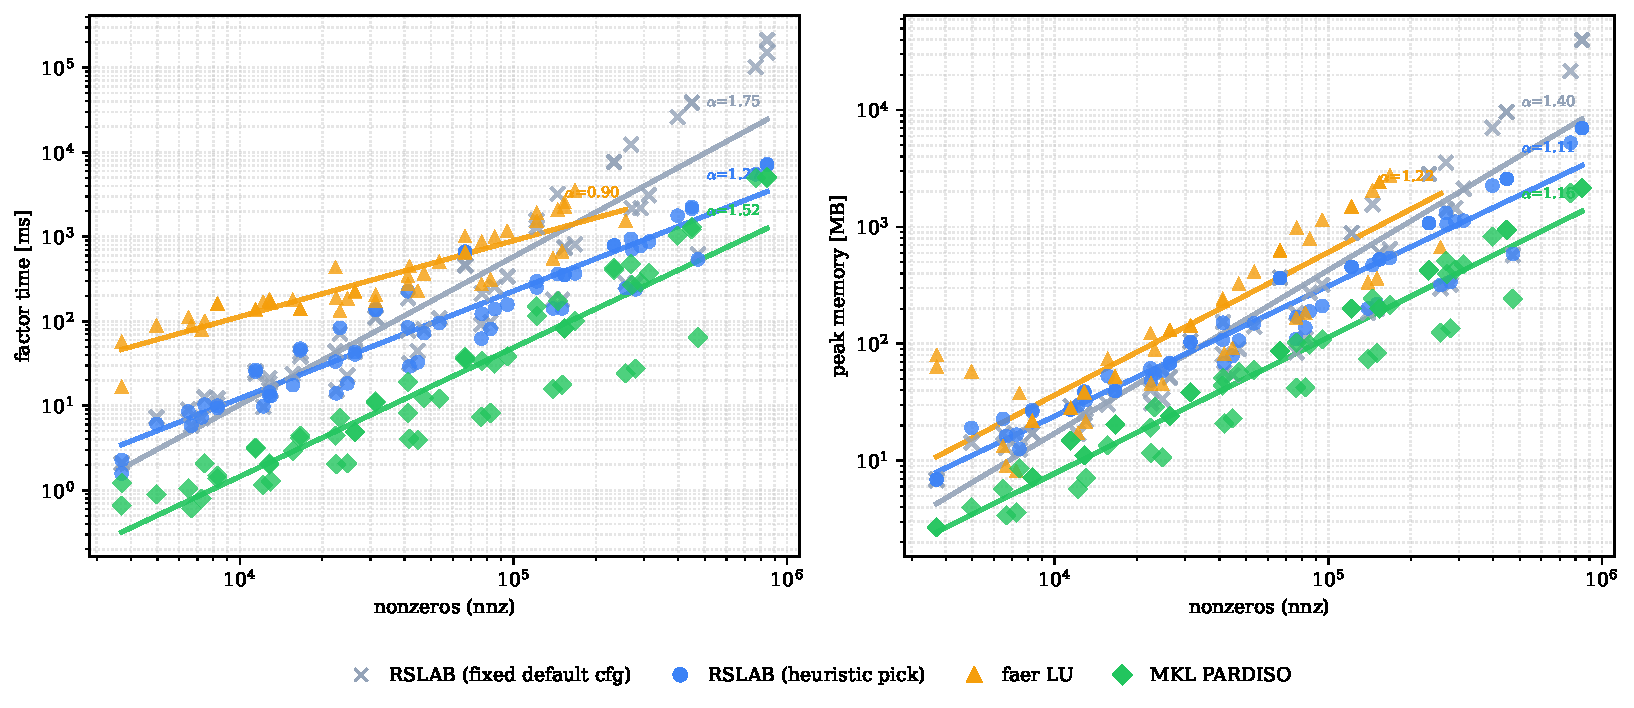
\includegraphics[width=\textwidth]{h2h_ldlt.pdf}
\caption{$\LDLt$ path (symmetric, PARDISO mtype 6): factor wall-clock (left) and peak
memory (right) vs.\ problem size: RSLAB vs.\ faer vs.\ MKL PARDISO, with power-law
fits.}
\label{fig:h2h_ldlt}
\end{figure}

\begin{figure}[htbp]
\centering
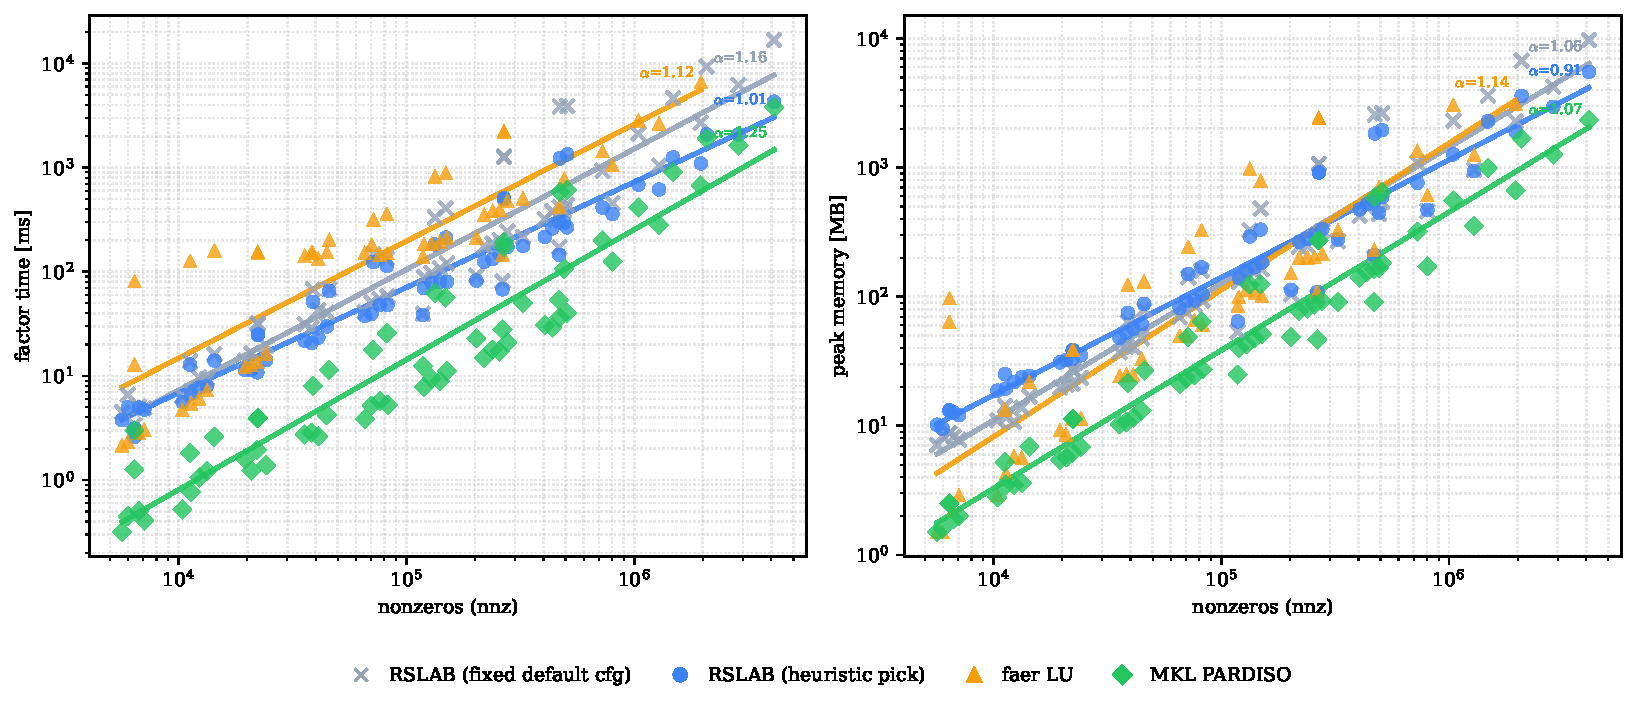
\includegraphics[width=\textwidth]{h2h_lu.pdf}
\caption{$\LU$ path (unsymmetric, PARDISO mtype 13): factor wall-clock (left) and peak
memory (right) vs.\ problem size. The fixed RSLAB default configuration (gray)
accompanies the heuristic pick (blue); on time the pick scales flatter than PARDISO
($\alpha\approx1.01$ vs.\ $1.25$).}
\label{fig:h2h_lu}
\end{figure}

\begin{table}[htbp]
\centering\tabfont
\begin{tabular}{@{}lcc@{}}
\toprule
RSLAB vs & $\LDLt$ (sym) & $\LU$ (unsym) \\
\midrule
MKL PARDISO: factor time & $5.6\times$ slower & $5.1\times$ slower \\
MKL PARDISO: peak memory & $2.8\times$ more & $3.6\times$ more \\
faer $\LU$\textsuperscript{$\dagger$}: factor time & \textbf{\num{6.7}}$\times$ faster & \textbf{\num{2.7}}$\times$ faster \\
faer $\LU$\textsuperscript{$\dagger$}: peak memory & \textbf{\num{1.8}}$\times$ less & $1.4\times$ more \\
fixed default cfg: factor time & \textbf{\num{1.84}}$\times$ faster & \textbf{\num{1.49}}$\times$ faster \\
fixed default cfg: peak memory & \textbf{\num{0.90}}$\times$ (less) & $1.11\times$ more \\
\bottomrule
\end{tabular}
\caption{Head-to-head geomean ratios (63 sizes per path, 1k--110k DOFs),
each path on its own class, over the matrices both solvers factor to below $0.1$
residual. The last rows are the shipped heuristic pick against the fixed RSLAB
default configuration. Unsym memory ratios above $1$ are the worker-count trade:
the calibrated pick runs more workers than the capped fixed config, raising the
transient panel peak.
\textsuperscript{$\dagger$}faer has no symmetric path (it factors symmetric matrices as
$\LU$), so its $\LDLt$ gap is structurally largest; it also OOMs on the largest
matrices, so its head-to-head is a conservative floor.}
\label{tab:scaling}
\end{table}

\begin{figure}[htbp]
\centering
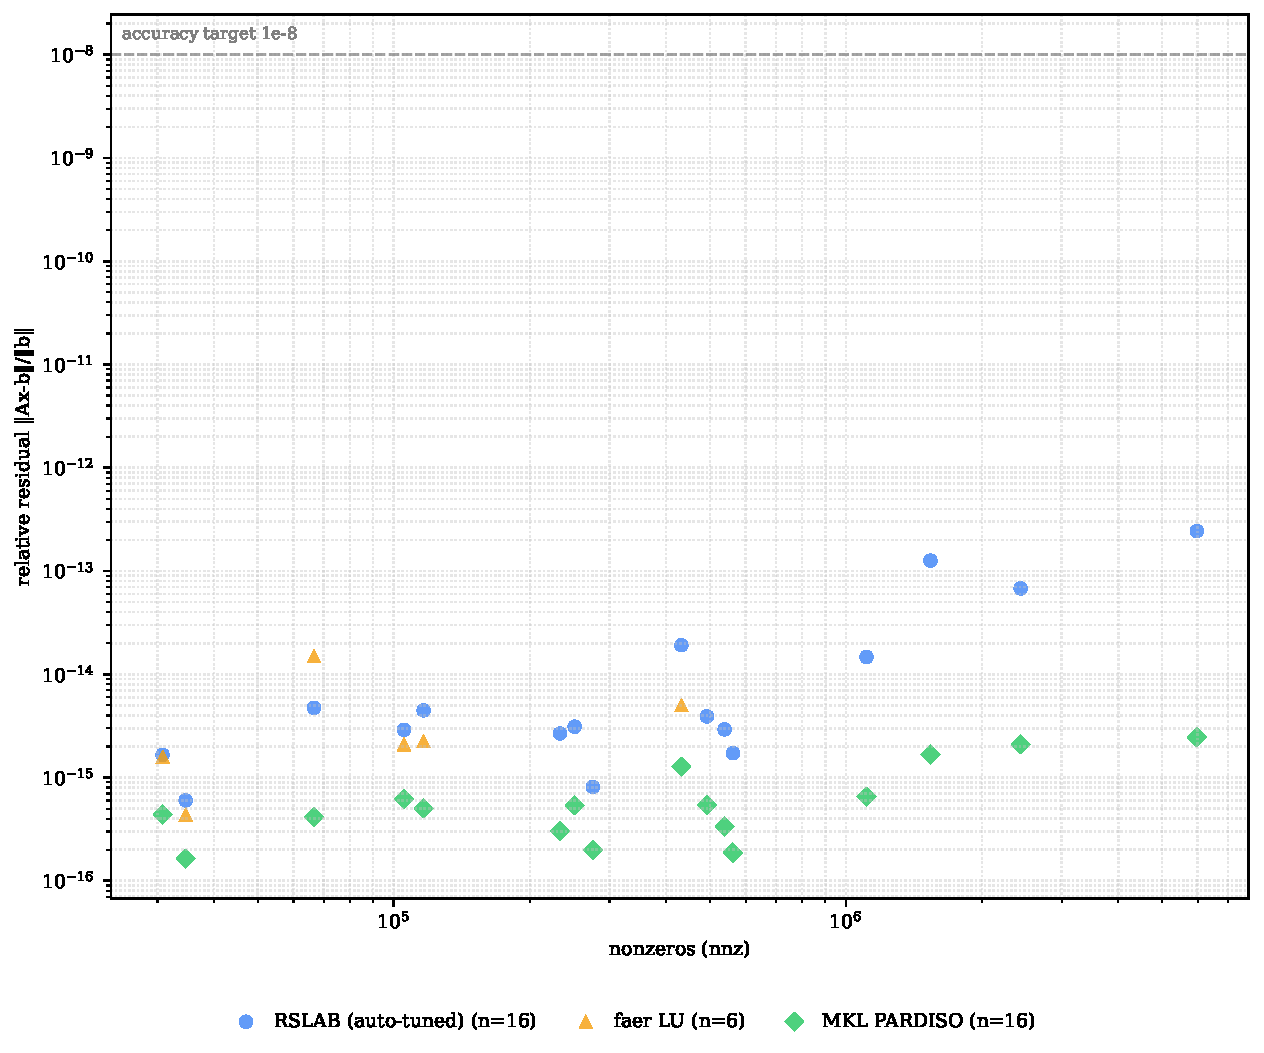
\includegraphics[width=\textwidth]{corpus_residual.pdf}
\caption{Relative residual $\|Ax-b\|/\|b\|$ across the corpus, per solver.}
\label{fig:residual}
\end{figure}

\subsection{Apple Silicon: \rT{} vs.\ Accelerate sparse solvers}
\label{sec:apple}
A second, independent measurement of all three solver paths on an Apple M3 (8 cores,
16\,GB, macOS 15.6) against Apple Accelerate's sparse direct solvers, which gained
complex support and a sparse LU in macOS 15.5. \rT{} runs its shipped default;
Accelerate runs its vendor-best configuration per class: Cholesky-first with an $\LDLt$
fallback for real-symmetric matrices, its sparse LU (TPP, \code{pivotTolerance} $0.01$)
for unsymmetric and circuit-shaped ones, and, because its complex $\LDLt$ is
Hermitian-only (verified empirically: the lower triangle is mirrored conjugated), LU on
the \emph{full} matrix for the complex-symmetric families, the same structural handicap
faer carries. Each matrix gets an AMD-vs-Metis ordering bakeoff
(\code{SparseOrderDefault} is plain AMD, up to $4.4\times$ the Metis fill on the large
EM/FEM systems); the bakeoff cost is charged to Accelerate's analyze time, mirroring
\rT's exact ordering race.

Results are reported as \emph{wall time divided by Accelerate's}, so $1.0$ is Accelerate
and lower is faster, under two metrics that answer different questions: \emph{factor
only} is the cost of a repeated factorization on a fixed pattern, \emph{one-shot} is
analyze plus factor plus solve, what a caller solving a single system waits for. Both
solvers race orderings inside their analyze, so the one-shot column compares like with
like. \rT's shipped thread policy caps at four workers while Accelerate uses all cores;
on the convection--diffusion class that cap costs \numrange{12}{17}\%. The numbers below
keep the shipped default.

\begin{figure}[htbp]
\centering
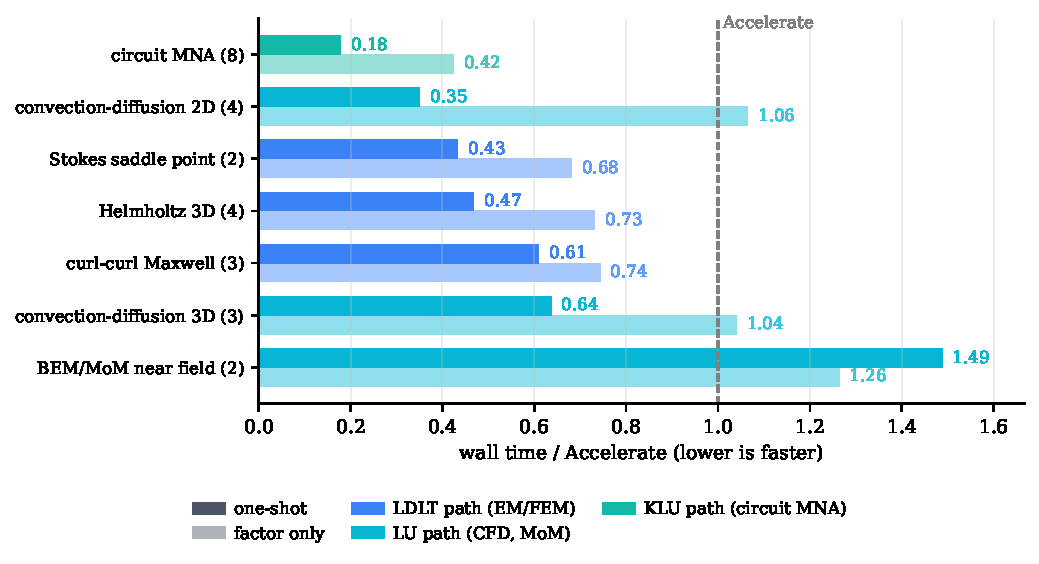
\includegraphics[width=0.92\textwidth]{accel_classes.pdf}
\caption{Apple M3, 8 threads: \rT{} v0.29 wall time divided by Accelerate's, per matrix
class, factor only and one-shot. Bars below $1.0$ are faster than the vendor library.}
\label{fig:apple_classes}
\end{figure}

\begin{table}[htbp]
\centering\tabfont
\begin{tabular}{@{}lcc@{}}
\toprule
matrix class & factor only & one-shot \\
\midrule
circuit MNA (KLU path) & \textbf{0.42} & \textbf{0.18} \\
Stokes saddle point & \textbf{0.68} & \textbf{0.43} \\
Helmholtz 3D & \textbf{0.73} & \textbf{0.47} \\
curl--curl Maxwell & \textbf{0.74} & \textbf{0.61} \\
convection--diffusion 3D & 1.04 & \textbf{0.64} \\
convection--diffusion 2D & 1.06 & \textbf{0.35} \\
BEM/MoM near field & 1.26 & 1.49 \\
\midrule
geomean over the three paths & \textbf{0.70} & \textbf{0.38} \\
\bottomrule
\end{tabular}
\caption{Apple M3 head-to-head, \rT{} wall time / Accelerate wall time (lower is
faster), over the matrices both solve to below $0.1$ residual. Nine sizes per generator
family on a 4k--110k log grid plus eight circuit sizes to 200k.}
\label{tab:apple}
\end{table}

The vendor's AMX-backed kernels own the small and mid sizes, and the ratio improves with
the problem: Helmholtz reaches $0.52$ at $n=\num{110592}$ and convection--diffusion 3D
$0.68$ at the same size (Fig.~\ref{fig:apple_scaling}). The circuit class stays below $0.45$ at every measured size. The one class behind on both metrics is the near-dense
BEM/MoM block, which is also the class where the analyze does not pay for itself. Its
fronts are medium-sized and near-dense, the regime where the packed complex GEMM runs at
a few GF/s against the \numrange{31}{40}\,GF/s it sustains on hot operands of the same
shape, because each update streams its operands once and reuses nothing.

\begin{figure}[htbp]
\centering
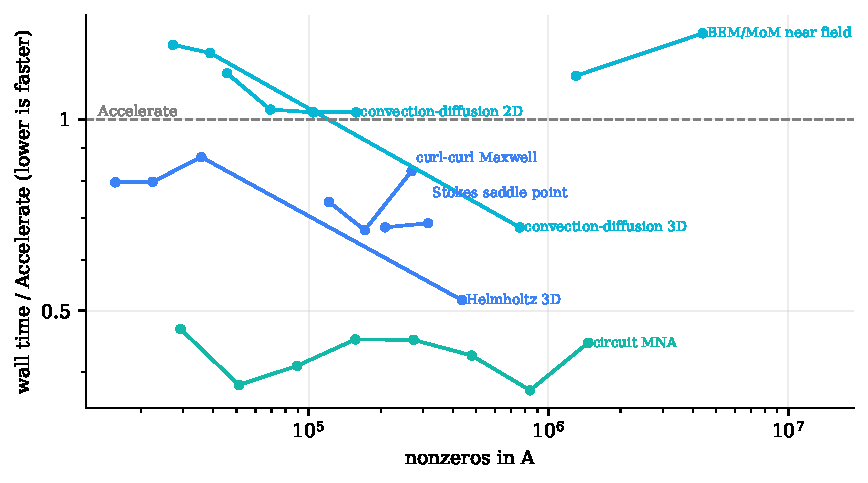
\includegraphics[width=0.85\textwidth]{accel_scaling.pdf}
\caption{Normalized wall time vs.\ problem size, one line per matrix class. Every class
improves with size; the two that end above $1.0$ are the ones whose fronts stay small
(convection--diffusion) or near-dense (BEM/MoM).}
\label{fig:apple_scaling}
\end{figure}

Measurement protocol: absolute times on this machine drift with its thermal state over a
long session, so each configuration pair is measured interleaved and reported as the
minimum over rounds, and Accelerate is re-measured in the same rounds as the solver it is
compared against.

On accuracy, Accelerate reaches $10^{-8}$ on 25 of 36 corpus matrices, but on five hard
indefinite/ill-scaled ones (stokes64, bratu3d, cont-201, rim, lhr34) it returns NaN or
garbage \emph{with an OK status}, the same silent-degradation mode as faer, where \rT{}
declines cleanly.

\subsection{KLU path on circuit-shaped matrices}
Table~\ref{tab:klu} benchmarks the KLU path against the multifrontal $\LU$ (defaults) on
MNA-like matrices: $\sim$4--5 nnz/column, unsymmetric, column-diagonally dominant,
cascaded stages giving a genuinely reducible BTF structure
(\code{cargo bench --bench klu\_circuit}, Apple M3). The KLU factor is
\numrange{5}{12}$\times$ faster with \numrange{1.7}{5.7}$\times$ less fill, the gap
widening with size as the multifrontal fronts grow; the numeric-only refactor runs
$\sim2\times$ faster still, so a 20-point sweep (refactor+solve vs.\ factor+solve) is
\numrange{10}{40}$\times$ faster end to end. Both solvers reach machine-precision
residuals ($\sim10^{-15}$) on every size. The shipped default runs the
independent BTF blocks in parallel once a deterministic structural gate clears
(at least 4 blocks, 8k nonzeros), bit-identical to the sequential result,
adding \numrange{3.1}{3.9}$\times$ on factor and \numrange{3.9}{4.5}$\times$
on refactor.

\begin{table}[htbp]
\centering\tabfont
\begin{tabular}{@{}rrrrrrrrr@{}}
\toprule
& & \multicolumn{4}{c}{KLU} & \multicolumn{2}{c}{multifrontal $\LU$} & \\
\cmidrule(lr){3-6}\cmidrule(lr){7-8}
$n$ & $\nnz$ & factor & refactor & fill & blocks & factor & fill & sweep ratio \\
\midrule
2k & 15k & \SI{1.7}{ms} & \SI{0.8}{ms} & 79k & 8 & \SI{8.1}{ms} & 132k & $9.8\times$ \\
10k & 73k & \SI{8.0}{ms} & \SI{4.1}{ms} & 439k & 16 & \SI{54.7}{ms} & 1.03M & $12.5\times$ \\
50k & 366k & \SI{45.4}{ms} & \SI{24.3}{ms} & 2.32M & 32 & \SI{304}{ms} & 9.21M & $13.9\times$ \\
200k & 1.47M & \SI{179}{ms} & \SI{96}{ms} & 9.17M & 64 & \SI{2.16}{s} & 52.2M & $40\times$ \\
\bottomrule
\end{tabular}
\caption{KLU vs.\ multifrontal $\LU$ on MNA-like circuit matrices (Apple M3). ``Sweep
ratio'' is the wall-clock ratio of 20 same-pattern value sets solved by KLU
refactor+solve vs.\ multifrontal factor+solve. Fill counts stored factor entries.}
\label{tab:klu}
\end{table}

Against the reference C implementation, SuiteSparse KLU~\cite{klu} (loaded at
runtime when installed), the analyze pipeline is at parity: identical BTF block
counts and fill within 1.5\% (\rT{} slightly less), confirming the maximum
transversal, Tarjan SCC, and per-block AMD match the reference. On the numeric
kernel (32-bit index streams, packed DFS marks, Eisenstat-Liu symmetric
pruning~\cite{eisenstatliu}, and a recorded refactor scatter program), the
sequential factor runs within \numrange{1.2}{1.6}$\times$ of the C code
(e.g.\ \SI{170}{ms} vs.\ \SI{135}{ms} at $n=200$k) and the refactor within
\numrange{1.15}{1.4}$\times$. The bit-identical parallel per-block
execution (the gated shipped default; factor and refactor; two-phase spliced
output) is
\numrange{1.6}{2.7}$\times$ \emph{faster} than SuiteSparse KLU on factor
and \numrange{2.1}{3.4}$\times$ on refactor (\SI{51}{ms} / \SI{24}{ms} at
$n=200$k), putting the 20-point sweep ${\sim}2.4\times$ ahead end to end.
Both reach $\sim10^{-15}$ residuals. On the real SuiteSparse circuit corpus the
column pipeline inside the dominant block (Sec.~\ref{sec:klu}) adds
\numrange{2.0}{2.9}$\times$ on refactor on the work-heavy matrices, where the block
structure is one large irreducible block that per-block parallelism cannot split.

\begin{figure}[htbp]
\centering
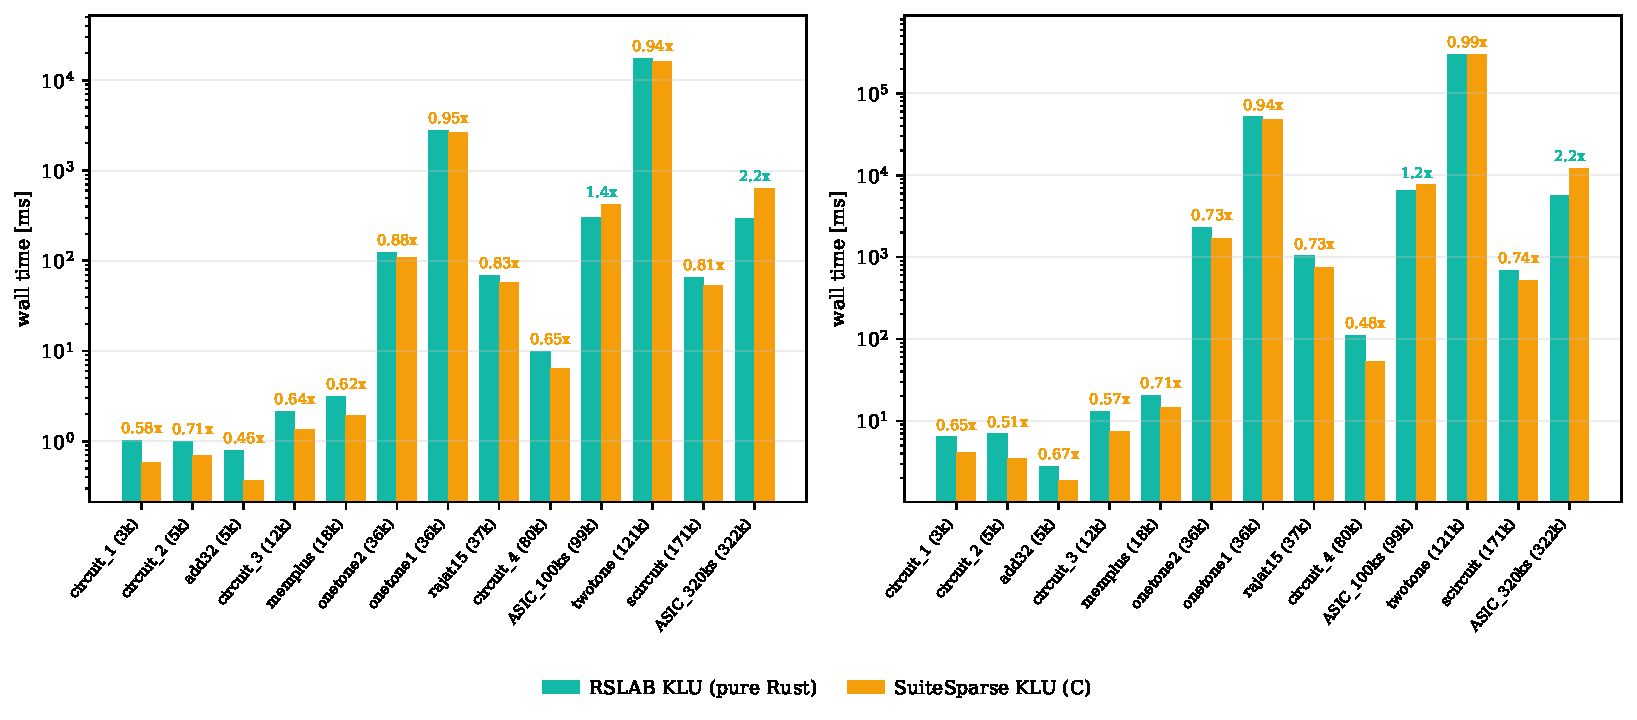
\includegraphics[width=\textwidth]{h2h_klu_realworld.pdf}
\caption{Real circuit matrices from the SuiteSparse collection: \rT{} KLU vs.\
SuiteSparse KLU, one pivoting factorization (left) and a 20-point same-pattern sweep of
refactor plus solve (right), log scale, labelled with the per-matrix ratio. The ratio is
matrix-dependent, spanning $0.47\times$ to $27.9\times$ on the factor and
$0.38\times$ to $25.8\times$ on the sweep.}
\label{fig:klu_realworld}
\end{figure}

\subsection{Iterative layer}
\begin{figure}[htbp]
\centering
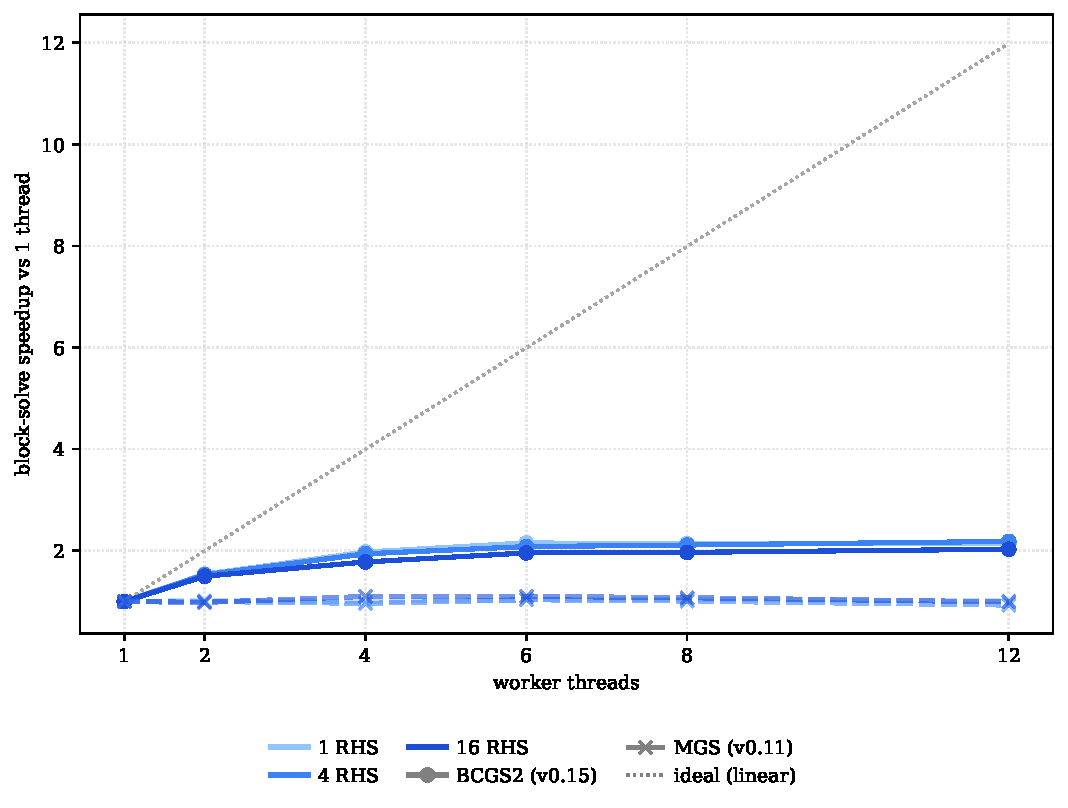
\includegraphics[width=0.62\textwidth]{block_gmres_scaling.pdf}
\caption{Strong scaling of the block solve against one worker, per block width, with the
per-RHS MGS path (dashed) for reference.}
\label{fig:blockgmres}
\end{figure}

\begin{figure}[htbp]
\centering
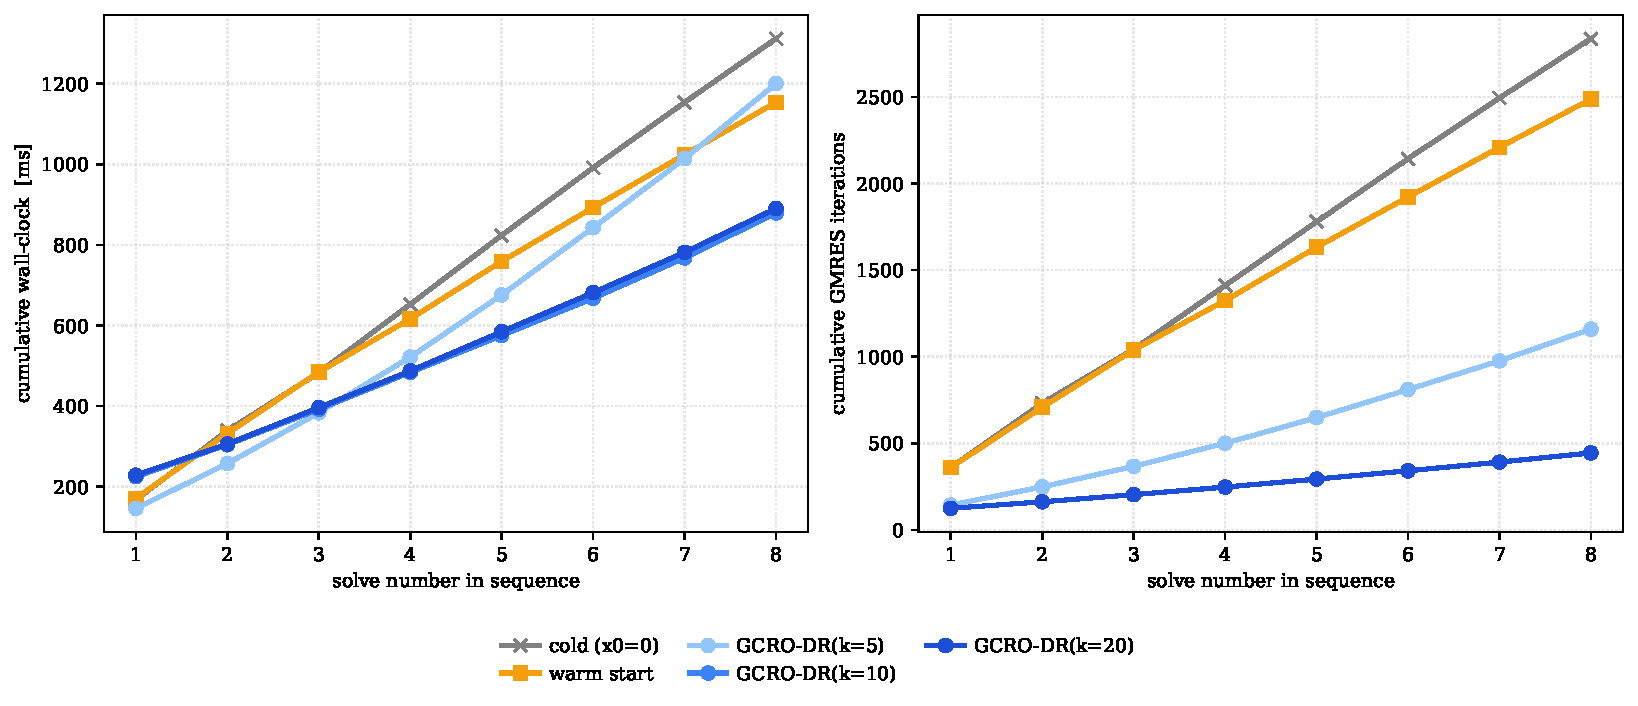
\includegraphics[width=\textwidth]{recycle_study.pdf}
\caption{A sequence of eight related solves: cumulative wall-clock (left) and cumulative
GMRES iterations (right), cold start vs.\ warm start vs.\ GCRO-DR recycling at three
subspace sizes.}
\label{fig:recycle}
\end{figure}

The Krylov results appear with their concepts in Sec.~\ref{sec:iterative}: block-CGS2
lifts multi-RHS strong scaling to $\sim2.2\times$ at 12 cores where per-RHS MGS is flat; within-cycle deflation cuts the batched operator
column-applies to $0.66\times$ the full-width bound at $s=16$; GCRO-DR recycling cuts
the cross-solve iteration total $6.4\times$ on a stagnating sequence; and the
incomplete-factor sweet spot at $\code{drop\_tol}=10^{-2}$ halves the factor memory at a
total wall time within a few percent of the exact direct solve. FGMRES's flexible-basis
update saves exactly one preconditioner solve per restart cycle, confirmed by counting.

\section{Conclusion}
\rT{} is a pure-Rust, scalar-generic sparse direct solver with three paths matched to
their operator classes: a supernodal complex-symmetric $\LDLt$, a supernodal/multifrontal
threshold-pivoted $\LU$, and a sequential, bit-deterministic KLU path with a numeric-only
refactor for fixed-pattern sweeps. It reaches within a single-digit factor of MKL PARDISO
while remaining dependency-free, is faster and leaner than the open-source alternatives,
and on Apple Silicon it factors the corpus in $0.70$ of Accelerate's wall time
($0.38$ one-shot) in geomean over the three paths. Its analyze phase computes memory,
work and runtime as exact functions of the structure, which is what lets the shipped
configuration be an exact race over candidates rather than a model of them. When the factor is made
approximate it becomes a preconditioner, and the matching Krylov layer (COCG/COCR,
flexible GMRES, deflating block GMRES, GCRO-DR recycling) turns the direct factor into
the engine of a fast preconditioned iterative solver.

\begingroup
\footnotesize
\setlength{\itemsep}{1pt}
\begin{thebibliography}{99}

\bibitem{amd} P.~R. Amestoy, T.~A. Davis, I.~S. Duff. An approximate minimum degree
ordering algorithm. \emph{SIAM J. Matrix Anal. Appl.} 17(4):886--905, 1996.

\bibitem{amf} P.~R. Amestoy. Recent progress in parallel multifrontal solvers and the
approximate minimum fill (HAMF) ordering. Technical report / CERFACS, 1999.

\bibitem{rothberg-minfill} E. Rothberg, S.~C. Eisenstat. Node selection strategies for
bottom-up sparse matrix ordering. \emph{SIAM J. Matrix Anal. Appl.} 19(3):682--695, 1998.

\bibitem{george} A. George. Nested dissection of a regular finite element mesh.
\emph{SIAM J. Numer. Anal.} 10(2):345--363, 1973.

\bibitem{metis} G. Karypis, V. Kumar. A fast and high quality multilevel scheme for
partitioning irregular graphs. \emph{SIAM J. Sci. Comput.} 20(1):359--392, 1998.

\bibitem{ssids} J.~D. Hogg, E. Ovtchinnikov, J.~A. Scott. A sparse symmetric indefinite
direct solver for GPU architectures (SSIDS). \emph{ACM Trans. Math. Softw.}
42(1):1--25, 2016.

\bibitem{ashcraft} C. Ashcraft, R. Grimes. The influence of relaxed supernode partitions
on the multifrontal method. \emph{ACM Trans. Math. Softw.} 15(4):291--309, 1989.

\bibitem{bunchkaufman} J.~R. Bunch, L. Kaufman. Some stable methods for calculating
inertia and solving symmetric linear systems. \emph{Math. Comp.} 31(137):163--179, 1977.

\bibitem{duffreid} I.~S. Duff, J.~K. Reid. The multifrontal solution of indefinite sparse
symmetric linear equations. \emph{ACM Trans. Math. Softw.} 9(3):302--325, 1983.

\bibitem{liumf} J.~W.~H. Liu. The multifrontal method for sparse matrix solution: theory
and practice. \emph{SIAM Review} 34(1):82--109, 1992.

\bibitem{liu86} J.~W.~H. Liu. On the storage requirement in the out-of-core multifrontal
method for sparse factorization. \emph{ACM Trans. Math. Softw.} 12(3):249--264, 1986.

\bibitem{umfpack} T.~A. Davis. Algorithm 832: UMFPACK, an unsymmetric-pattern
multifrontal method. \emph{ACM Trans. Math. Softw.} 30(2):196--199, 2004.

\bibitem{eisenstatliu} S.~C. Eisenstat, J.~W.~H. Liu. Exploiting structural symmetry in
unsymmetric sparse symbolic factorization. SIAM J. Matrix Anal. Appl., 13(1), 1992.
\bibitem{klu} T.~A. Davis, E. Palamadai Natarajan. Algorithm 907: KLU, a direct sparse
solver for circuit simulation problems. \emph{ACM Trans. Math. Softw.} 37(3):36, 2010.

\bibitem{carsonhigham} E. Carson, N.~J. Higham. Accelerating the solution of linear
systems by iterative refinement in three precisions. \emph{SIAM J. Sci. Comput.}
40(2):A817--A847, 2018.

\bibitem{hopcroftkarp} J.~E. Hopcroft, R.~M. Karp. An $n^{5/2}$ algorithm for maximum
matchings in bipartite graphs. \emph{SIAM J. Comput.} 2(4):225--231, 1973.

\bibitem{nicslu} X. Chen, Y. Wang, H. Yang. NICSLU: an adaptive sparse matrix solver for
parallel circuit simulation. \emph{IEEE Trans. CAD} 32(2):261--274, 2013.

\bibitem{pardiso} O. Schenk, K. G\"artner. Solving unsymmetric sparse systems of linear
equations with PARDISO. \emph{Future Gener. Comput. Syst.} 20(3):475--487, 2004.

\bibitem{faer} S. Quinones. faer-rs: a linear algebra library for the Rust programming
language. \url{https://github.com/sarah-quinones/faer-rs}, 2024.

\bibitem{suitesparse} T.~A. Davis, Y. Hu. The University of Florida sparse matrix
collection. \emph{ACM Trans. Math. Softw.} 38(1):1--25, 2011.

\bibitem{saadschultz} Y. Saad, M.~H. Schultz. GMRES: a generalized minimal residual
algorithm for solving nonsymmetric linear systems. \emph{SIAM J. Sci. Stat. Comput.}
7(3):856--869, 1986.

\bibitem{fgmres} Y. Saad. A flexible inner--outer preconditioned GMRES algorithm.
\emph{SIAM J. Sci. Comput.} 14(2):461--469, 1993.

\bibitem{dgks} J.~W. Daniel, W.~B. Gragg, L. Kaufman, G.~W. Stewart. Reorthogonalization
and stable algorithms for updating the Gram--Schmidt QR factorization. \emph{Math. Comp.}
30(136):772--795, 1976.

\bibitem{giraud} L. Giraud, J. Langou, M. Rozlo\v{z}n\'ik, J. van den Eshof. Rounding
error analysis of the classical Gram--Schmidt orthogonalization process. \emph{Numer.
Math.} 101(1):87--100, 2005.

\bibitem{barlow} J.~L. Barlow, A. Smoktunowicz. Reorthogonalized block classical
Gram--Schmidt. \emph{Numer. Math.} 123(3):395--423, 2013.

\bibitem{gcrodr} M.~L. Parks, E. de~Sturler, G. Mackey, D.~D. Johnson, S. Maiti.
Recycling Krylov subspaces for sequences of linear systems. \emph{SIAM J. Sci. Comput.}
28(5):1651--1674, 2006.

\bibitem{morgan} R.~B. Morgan. GMRES with deflated restarting. \emph{SIAM J. Sci.
Comput.} 24(1):20--37, 2002.

\bibitem{cocg} H.~A. van der Vorst, J.~B.~M. Melissen. A Petrov--Galerkin type method
for solving $Ax=b$, where $A$ is symmetric complex. \emph{IEEE Trans. Magn.}
26(2):706--708, 1990.

\bibitem{cocr} T. Sogabe, S.-L. Zhang. A COCR method for solving complex symmetric
linear systems. \emph{J. Comput. Appl. Math.} 199(2):297--303, 2007.

\end{thebibliography}
\endgroup

\end{document}
